\documentclass{projetofinal-dcc}
%%%%%%%%%%%%%%%%%%%%%%%%%%%%%%%%%%%%%%%%%%%%%%%%%%%%%%%%%%%%
%P A C O T E S
%%%%%%%%%%%%%%%%%%%%%%%%%%%%%%%%%%%%%%%%%%%%%%%%%%%%%%%%%%%%
% Adicione aqui seus pacotes

%%%%%%%%%%%%%%%%%%%%%%%%%%%%%%%%%%%%%%%%%%%%%%%%%%%%%%%%%%%%
%I N I C I O  D O  D O C U M E N T O
%%%%%%%%%%%%%%%%%%%%%%%%%%%%%%%%%%%%%%%%%%%%%%%%%%%%%%%%%%%%
\begin{document}

% título da tese é obrigatório
\title{You Can Test: Desenvolvimento ágil de uma ferramenta de testes automatizados na nuvem para sistemas em produção}

% autor é obrigatório; máximo de 3 autores
\author{Guilherme Miranda Moreira Bomfim}{\input{elementos-pretextuais/agradecimentos}}
\author{Rebeca Beatriz Maciel Bordini}{\input{elementos-pretextuais/agradecimentos}}
%\author{Nome completo aluno 3}{\input{elementos-pretextuais/agradecimentos}}

% orientador é obrigatório
\advisor[Prof.]{Rodrigo Penteado Ribeiro de Toledo, ~Ph.D.}{}

% co-orientador é opcional
\coadvisor[Prof.]{Carlos Felippe Cardoso de Resende, ~M.Sc.}{}

% máximo de 3 integrantes da banca (orientador e co-orientador já são adicionados automaticamente)
\banca[Prof.]{Nome do participante banca 1,~D.Sc.}{COPPE~-~UFRJ}
\banca[Prof.]{Nome do participante banca 2,~Ph.D.}{COPPE~-~UFRJ}
%\banca[Prof.]{Nome do participante banca 3,~Ph.D.}{COPPE~-~UFRJ}

\location{Rio~de~Janeiro}{RJ}{Brasil}

% mês e ano de defesa
\date{Janeiro}{2015}
\maketitle

\startdocument
%%%%%%%%%%%%%%%%%%%%%%%%%%%%%%%%%%%%%%%%%%%%%%%%%%%%%%%%%%%%
%A G R A D E C I M E N T O S
%%%%%%%%%%%%%%%%%%%%%%%%%%%%%%%%%%%%%%%%%%%%%%%%%%%%%%%%%%%% 
\makethankspage

%%%%%%%%%%%%%%%%%%%%%%%%%%%%%%%%%%%%%%%%%%%%%%%%%%%%%%%%%%%%
%R E S U M O
%%%%%%%%%%%%%%%%%%%%%%%%%%%%%%%%%%%%%%%%%%%%%%%%%%%%%%%%%%%%
\begin{abstract}{
  No contexto de desenvolvimento de aplicações, muitas vezes nós, como desenvolvedores destas e/ou responsáveis pela sua manutenção, nos deparamos com situações onde existe muito interesse em desenvolver testes automatizados para o projeto, mas há muitos empecilhos que no dia-a-dia nos impedem de aplicar essa prática no nosso cotidiano. 

Dado em vista que para começar a desenvolver testes automatizados para a sua aplicação a curva de aprendizado é alta, realizamos um estudo de caso com diversas comunidades de desenvolvedores para que pudéssemos identificar quais são as dificuldades em adotar essa prática, e como podíamos encontrar uma forma de auxiliá-los a incorporar a prática de testes no seu ambiente de trabalho trazendo um alto ROI(Return Over Investiment) entregando testes de valor de forma rápida e fácil.

O objetivo desse trabalho foi criar uma aplicação onde seria possível realizar testes da aplicação já em produção, na nuvem. De forma rápida e sem precisar codificar.
}
\end{abstract}

%%%%%%%%%%%%%%%%%%%%%%%%%%%%%%%%%%%%%%%%%%%%%%%%%%%%%%%%%%%%
%A B S T R A C T
%%%%%%%%%%%%%%%%%%%%%%%%%%%%%%%%%%%%%%%%%%%%%%%%%%%%%%%%%%%%
\begin{englishabstract}{
  \input{elementos-pretextuais/abstract}
}
\end{englishabstract}

%%%%%%%%%%%%%%%%%%%%%%%%%%%%%%%%%%%%%%%%%%%%%%%%%%%%%%%%%%%%
%L I S T A S
%%%%%%%%%%%%%%%%%%%%%%%%%%%%%%%%%%%%%%%%%%%%%%%%%%%%%%%%%%%%
% Figuras
\makefigurespage

% Tabelas
\maketablespage

% Algoritmos
\makelistingspage

% Abreviaturas (devem estar em ordem alfabética)
\makeabrevpage{\input{elementos-pretextuais/abreviaturas}}

% Símbolos (devem estar em ordem alfabética)
\makesymbolspage{\input{elementos-pretextuais/simbolos}}

% Sumário 
\maketocpage

%%%%%%%%%%%%%%%%%%%%%%%%%%%%%%%%%%%%%%%%%%%%%%%%%%%%%%%%%%%%
%C O N T E Ú D O
%%%%%%%%%%%%%%%%%%%%%%%%%%%%%%%%%%%%%%%%%%%%%%%%%%%%%%%%%%%%
\startcontent
\chapter{Introdução}\label{chp:LABEL_CHP_1}

\section{Motivação}\label{sec:LABEL_CHP_1_SEC_A}

Nos dias de hoje, em que a utilização da internet está cada vez maior, nos deparamos com usuários de diferentes níveis estão tomando parte no mundo digital. Neste cenário, temos cada vez mais sistemas web disponíveis na rede e interesses individuais naquele produto permanecer no ar. Mas será que esse interesse não deveria vir acompanhado com uma necessidade em manter essas aplicações testadas? Quando um cliente solicita para uma empresa que esta desenvolva o seu projeto, depois dele pronto, após alguns meses como o cliente saberá que não existem páginas retornando 404? Páginas com erro? Ou até mesmo o sistema não está disponível?! Foram a partir dessas necessidades que surgiu a motivação do projeto. 

Temos além disso desenvolvedores responsáveis pela manutenção de alguns desses códigos "legados", que não foram eles que desenvolveram mas que está na mão deles para a sua manutenção. Para identificar que esse cenário realmente ocorria na vida real realizamos uma análise dentro do mercado de desenvolvimento no Brasil. Nos utilizamos de fóruns e grupos de desenvolvedores no Facebook para aplicar pesquisas e assim determinar se essa análise era correta e identificava uma fatia real dos desenvolvedores brasileiros.


\chapter{Validação}\label{chp:LABEL_CHP_2}

Uma dificuldade que muitos alunos encontram na hora de escolher um tema para o projeto final para o curso de Graduação em Ciência da Computação é que, muitas vezes, não apenas desejam desenvolver um sistema que seja aplicável para a realização da sua colação de grau. Mas que o tema escolhido também possua uma aplicação com valor de negócio agregado e que seja utilizável por usuários realmente interessados e motivados.

Com essa preocupação, buscamos encontrar formas responsáveis de iniciar esse novo projeto, entendendo que seria necessário transformar a incerteza, de que teríamos um interesse significativo do público, em uma certeza. Para isso, antes de investir qualquer tempo no desenvolvimento dessa aplicação, buscamos encontrar uma forma de validar a nossa ideia inicial, de que construir um sistema para realizar testes de qualquer aplicação em produção na nuvem, era realmente uma ideia válida.

Existem diversas ferramentas que andam lado a lado com esse objetivo e ajudam a estruturar esse tipo de projeto, a que foi utilizada no projeto foi o Validation Board\cite{art:REF_ART_1}. Se trata em acompanhar o progresso do produto e focar no que realmente importa para o mesmo. É uma forma muito simples de descobrir se uma ideia vai funcionar ou se ela simplesmente não é válida, sendo totalmente baseada em ações e resultados rápidos.

\section{Validation Board}\label{sec:LABEL_CHP_2_SEC_A}

\begin{figure}
  \centering
  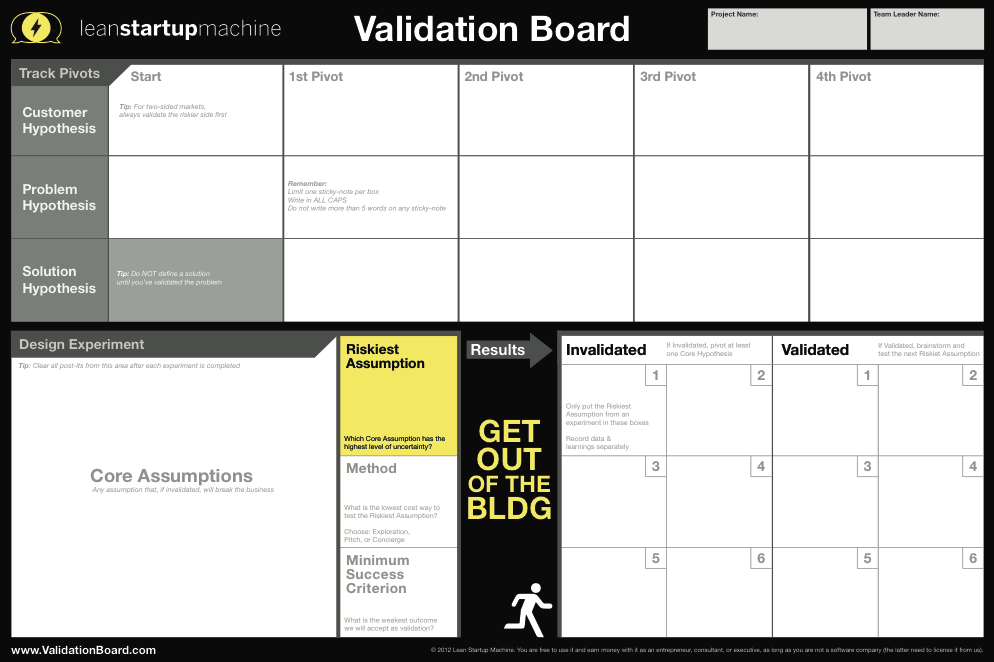
\includegraphics[width=0.6\textwidth]{imagens/validationTemplate.png}
  \caption{Validation Board}
  \label{fig:LABEL_FIG_1}
\end{figure}

O Validation Board foi desenvolvido pelo Lean Startup Machine, movimento formado por empreendedores do mundo todo que promove workshops de três dias que visa ensinar a construir algo que clientes tenham vontade de obter e também ensinam a executar experimentos que levem a sua empresa na direção certa. Ele é uma ferramenta simples e gratuita de testar as suas ideias, baseado na metodologia Lean\cite{art:REF_ART_2}.

O Validation Board consiste em criar hipóteses de determinado problema e de pessoas que sofrem do mesmo, gerando assim experimentos de constatação, ou não, dessas hipóteses. O objetivo é conseguir gerar aprendizado a partir da execução de cada um desses experimentos iterativamente, buscando sempre invalidar as hipóteses de maior para o menor risco, como por exemplo nos casos em que poderiam arruinar a ideia do seu produto.

Ao final de cada uma dessas iterações, temos dois resultados possíveis: a validação ou a invalidação da hipótese, e assim teremos insumos para tomar a próxima ação.

\subsection{A Hipótese}

O processo de validação é iniciado pelo topo do board, onde há espaço para diferentes pivôs. Pivôs são mudanças bruscas que não podem ocorrer na vida útil do produto no qual estamos aplicando esse processo. Primeiro definimos as hipóteses, são num total de três: Público Alvo, Problema e Solução. O público-alvo pode ser pensado como o grupo de pessoas que possui uma característica em comum. O problema deverá ser algo específico que esse grupo anterior possui. A solução é deixada em branco nessa primeira etapa. De forma a não ocultar outras  melhores oportunidades para resolver aquele problema. 

\subsection{Experimentações}

Na parte inferior do quadro, encontra-se a área de experimentação. Temos duas áreas: a de suposições iniciais onde deverão se encontrar as suposições que levam a acreditar que, se falharem, poderiam levar ao fracasso de todo o projeto; e a área de suposição de maior risco, que é a suposição a ser validada nessa iteração do processo.

\subsubsection {Métodos de teste}

A partir da suposição de maior risco, deve ser aplicado um experimento para provar a validade dessa suposição. Existem três métodos para isso:

\textbf{Exploration:} Neste método, o objetivo consiste em ir para as ruas e tentar reproduzir o problema que foi suposto na hipótese. Esse problema é algo real? Existem formas de resolvê-lo? Quais? Podem ser realizadas entrevistas com os usuários em potencial para, assim, identificar quais são as ideias que eles possuem a respeito de outras possíveis soluções para o problema também. Qualquer uma dessas atividades servem para prover insumos na hora de criar uma solução.

\textbf{Pitch:} O objetivo deste consiste no avaliador expor a ideia proposta para solucionar o problema e obter feedback dos usuários em potencial. De forma a descobrir o quanto eles pagariam, se pagariam, por utilizar essa solução e quanto.

\textbf{Concierge:} Este último método visa entregar ao cliente a sua hipótese de solução com a menor quantidade possível de desenvolvimento, de forma a fazê-los motivados com o produto que você tem a oferecer.

\subsubsection {Critério mínimo de sucesso}
Depois de definir qual será o método de teste a ser utilizado, é necessário definir quais serão os critérios que irão validar a sua ideia de fato, é muito importante que estes sejam definidos antes da aplicação do teste, para não viciar os seus resultados.

\subsection {Resultados}
Após toda a etapa de definição, deve-se "sair do prédio"  e realizar os experimentos necessários para a validação das premissas, conversando com pessoas reais de forma a por em prática o método de teste definido. 

A próxima fase consiste em determinar se os resultados alcançaram ou não o critério mínimo de sucesso, movendo a suposição para o campo validado ou invalidado. Caso ela seja invalidada, pode-se pivotar as hipóteses e reuniciar todo o processo. Caso contrário, o processo pode ser reiniciado com a próxima hipótese de maior risco, caso exista.

\section{Aplicação do Validation Board}\label{sec:LABEL_CHP_2_SEC_B}

Com o Validation Board, desejávamos validar se o problema que estávamos buscando solucionar era realmente um problema, então seguimos as etapas da seguinte forma:

\subsection{Definião das hipóteses}
Definimos as três hipóteses: público alvo, problema e solução.

\textbf {Público alvo:} Grupo de desenvolvedores que tenham vontade em testar seus sistemas.

\textbf {Problema:} O grupo de desenvolvedores deseja testar seus sistemas mas possui algum empecilho.

\textbf{Solução:} Não definimos essa hipótese para não deixarmos de visualizar alguma outra possível solução para o problema.

\subsection{Definição das suposições}

Além das hipóteses, foram definidas suposições que nos levavam a acreditar que se falhassem, levariam ao fracasso da nossa ideia.

\textbf{Suposições iniciais:}
\begin{itemize}
\item É difícil configurar um ambiente de testes;
\item O custo de criar testes em projetos pequenos é alto;
\item O desenvolvedor não possui um ambiente próprio para executar os testes localmente;
\end{itemize}

\textbf{Suposição de maior risco:}
Desenvolvedores querem testar seus sistemas com uma ferramenta disponível na nuvem.

\begin{figure}
  \centering
  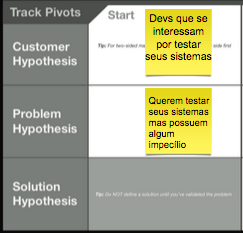
\includegraphics[width=0.6\textwidth]{imagens/hyphotesis.png}
  \caption{Hipóteses definidas no Validation Board}
  \label{fig:LABEL_FIG_2}
\end{figure}

\begin{figure}
  \centering
  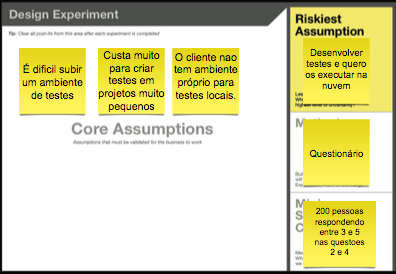
\includegraphics[width=0.6\textwidth]{imagens/assumptions.png}
  \caption{Suposições definidas no Validation Board}
  \label{fig:LABEL_FIG_3}
\end{figure}

\begin{figure}
  \centering
  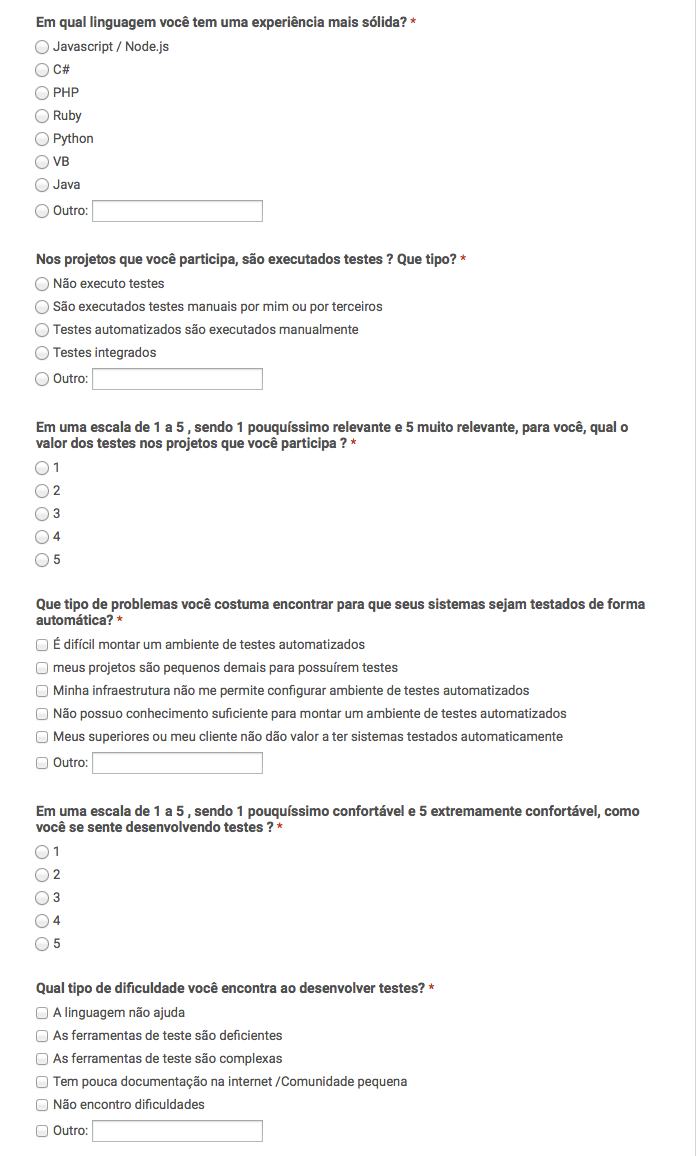
\includegraphics[width=0.8\textwidth]{imagens/survey.png}
  \caption{Pesquisa aplicada ao público alvo}
  \label{fig:LABEL_FIG_4}
\end{figure}

\subsection{Experimentação}

Para realizar as nossas experimentações, definimos o método de teste \emph{Exploration}, onde criamos um formulário com perguntas a serem aplicadas nos nossos possíveis clientes. Utilizamos como canal de aplicação desse formulário grupos de desenvolvedores no Facebook (NodeJS Brasil, Angular Brasil, Javascript Brasil, Javascript Brasil, etc).

\subsubsection{Aplicação}
A pesquisa foi formulada com um conjunto de perguntas que julgamos interessantes para identificar o perfil do desenvolvedor brasileiro, e por consequência, validar a nossa hipótese.

\textbf{Perguntas do formulário aplicado:}
\begin{enumerate}
\item Em qual linguagem o desenvolvedor possuia experiência mais sólida;
\item Se nos projetos em que o desenvolvedor participava, eram executados testes e de que tipo;
\item Qual o valor que o desenvolvedor dava a possuir testes nos seus projetos;
\item Quais eram os tipos de problemas que ele costumava enfrentar na hora de desenvolver alguma forma de automatização desses testes;
\item Qual era o nível de conforto que ele sentia na hora de desenvolver os testes no seu projeto;
\item Quais eram as dificuldades que ele encontrava para desenvolver testes automatizados
\end{enumerate}

\subsubsection{Critério mínimo de sucesso}
A partir dessas perguntas, mapeamos que para que a nossa hipótese fosse validada seria necessário que atingíssemos os seguintes critérios:

\begin{itemize}
\item Conseguir que, no mínimo, 40 desenvolvedores respondessem ao questionário;
\item Dentre esses desenvolvedores, no mínimo 60\% deveria responder que achava relevante, muito relevante ou extremamente relevante o valor dos testes nos projetos em que participavam
\item Além disso, no mínimo 60\% dos desenvolvedores não deveriam se sentir suficientemente confortáveis para desenvolver seus próprios testes
\end{itemize}

\subsection {Resultados}
Após a aplicação do método de exploração, conseguimos, com o auxílio da divulgação da pesquisa em grupos de desenvolvedores no Facebook, 204 resultados; o que satisfez o nosso primeiro critério. Quanto aos outros resultados quantitativos percebemos que:

\begin{itemize}
\item 86\% dos entrevistados consideravam o uso de testes em projetos relevante;
\item 62\% dos entrevistados não se sentem suficientemente confortáveis para desenvolver seus próprios testes
\end{itemize}

Com esses resultados, validamos a nossa hipótese de maior risco. De forma a também nos permitir adquirir um número maior de informação qualitativa sobre as dificuldades que esse público alvo possui em comum, o que serviu de insumos extras para o desenvolvimento da nossa aplicação. Dentre eles:

\begin{itemize}
\item 50\% dos projetos em que os entrevistados participaram, eram executados testes manuais pelos próprios ou por terceiros;
\item Somente 18\% dos desenvolvedores possuiam uma infra-estrutura para executar testes integrados;
\item Mais de $\frac{1}{3}$ dos entrevistados afirmaram que era difícil montar um ambiente de testes automatizados, e outro $\frac{1}{3}$ não possui conhecimento para configurar um;
\item 40\% desses desenvolvedores possuem superiores ou clientes que não dão valor a ter sistemas testados automaticamente  
\end{itemize}

\begin{figure}
  \centering
  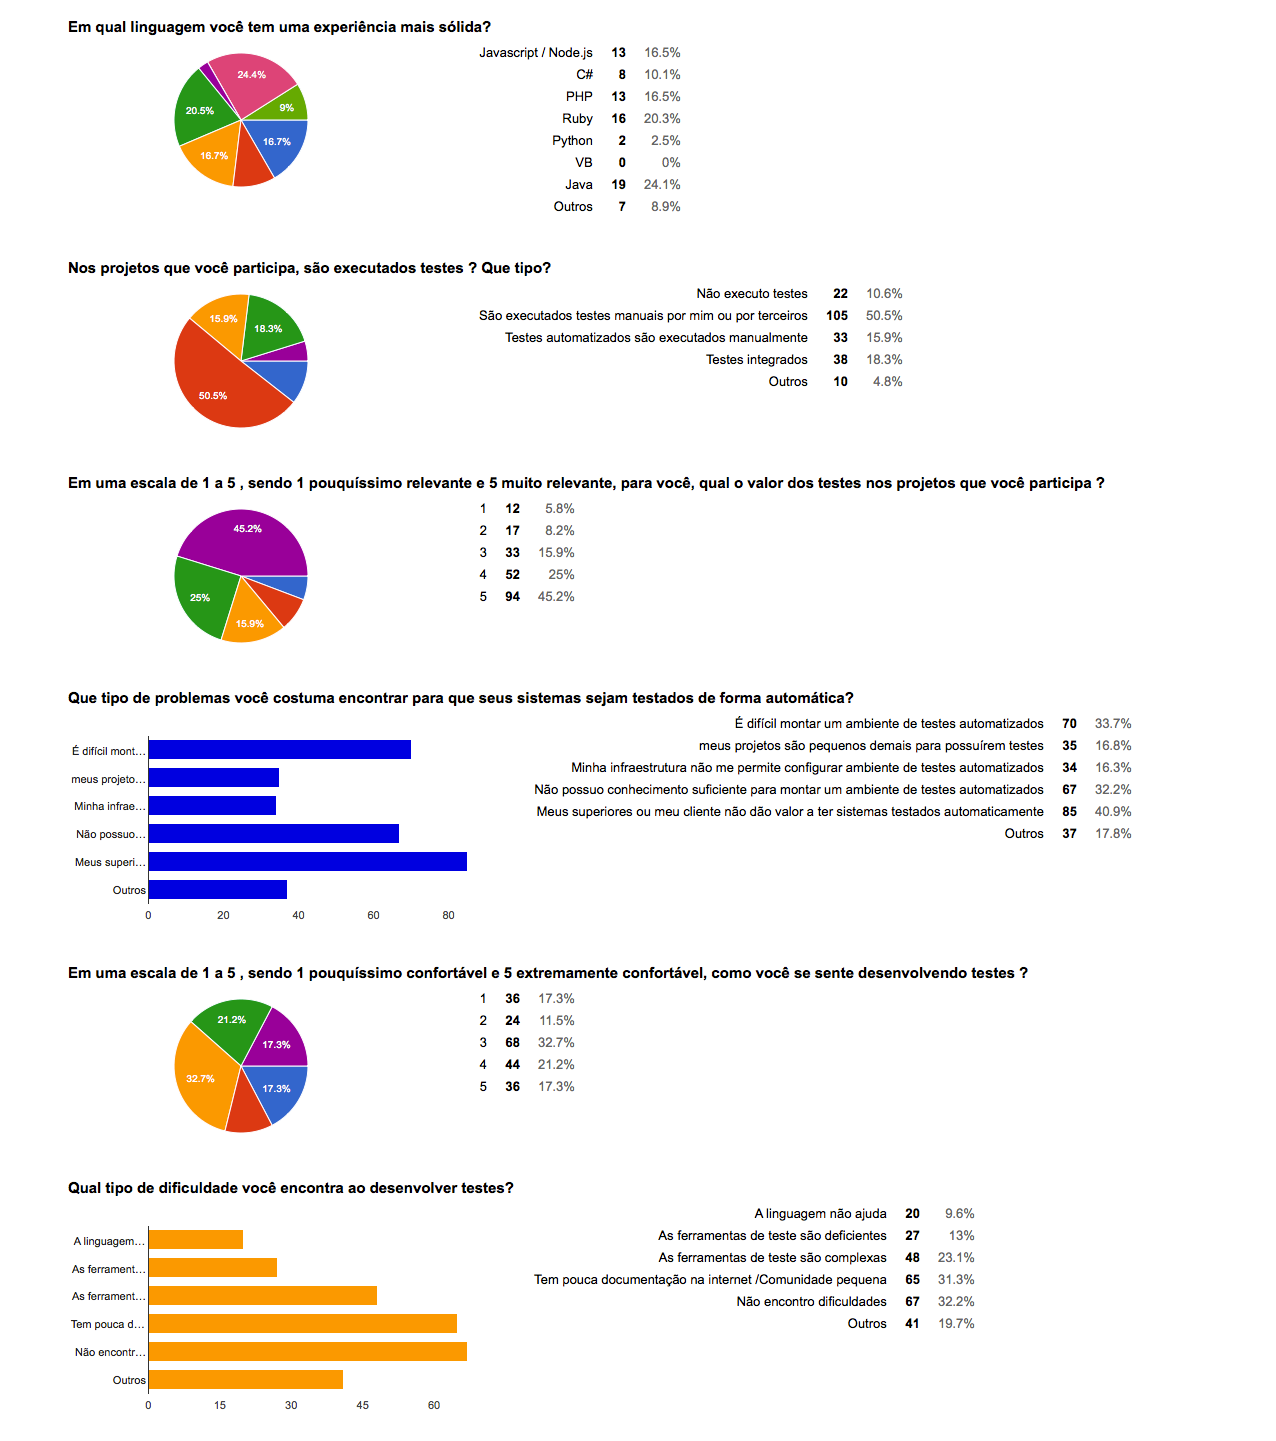
\includegraphics[width=1.1\textwidth]{imagens/results.png}
  \caption{Resultados da pesquisa aplicada}
  \label{fig:LABEL_FIG_5}
\end{figure}

Podemos perceber que o Validation Board serviu como uma ótima opção para testar a nossa ideia, visto que ele torna possível acertar o quanto antes se o caminho a ser seguido é realmente o melhor, ou não.

\pagebreak

%%%%%%%%%%%%%%%%%%%%%%%%%%%%%%%%%%%%%%%%%%%%%%%%%%%%%%%%%%%%
% B I B L I O G R A F I A
%%%%%%%%%%%%%%%%%%%%%%%%%%%%%%%%%%%%%%%%%%%%%%%%%%%%%%%%%%%%
% Retirar esta parte se o trabalho não tiver bibliografia
\makebibspage{abnt}{elementos-postextuais/referencias}

%%%%%%%%%%%%%%%%%%%%%%%%%%%%%%%%%%%%%%%%%%%%%%%%%%%%%%%%%%%%
% A P E N D I C E
%%%%%%%%%%%%%%%%%%%%%%%%%%%%%%%%%%%%%%%%%%%%%%%%%%%%%%%%%%%%
% Retirar esta parte se o trabalho não tiver anexos
\appendix
\input{elementos-postextuais/apendice}

\end{document}